\documentclass[conference]{IEEEtran}
\IEEEoverridecommandlockouts

% ==================== PACKAGES ====================
\usepackage[T1]{fontenc}
\usepackage{cite}
\usepackage{amsmath,amssymb,amsfonts}
\usepackage{graphicx}
\usepackage{textcomp}
\usepackage{xcolor}
\usepackage{booktabs}
\usepackage{multirow}
\usepackage{url}
\usepackage{microtype}
\usepackage{balance}
\usepackage{enumitem}
\usepackage[colorlinks=true,linkcolor=blue,citecolor=blue,urlcolor=blue]{hyperref}


% Standard balanced layout tuning for strict 7-page IEEE conference format
\setlist{nosep,leftmargin=*}
\setlength{\parskip}{0pt}
\setlength{\abovedisplayskip}{3pt plus 1pt minus 1pt}
\setlength{\belowdisplayskip}{3pt plus 1pt minus 1pt}
\setlength{\abovedisplayshortskip}{1.5pt plus 1pt}
\setlength{\belowdisplayshortskip}{1.5pt plus 1pt}
\setlength{\textfloatsep}{5pt plus 1pt minus 1pt}
\setlength{\floatsep}{4pt plus 1pt minus 1pt}
\setlength{\intextsep}{4pt plus 1pt minus 1pt}

% Float placement optimization
\renewcommand{\topfraction}{0.95}
\renewcommand{\bottomfraction}{0.95}
\renewcommand{\textfraction}{0.05}
\renewcommand{\floatpagefraction}{0.85}
\renewcommand{\dbltopfraction}{0.95}
\renewcommand{\dblfloatpagefraction}{0.85}
\setcounter{topnumber}{3}
\setcounter{bottomnumber}{2}
\setcounter{totalnumber}{5}

% Bibliography item spacing tuning
\let\oldthebibliography\thebibliography
\let\endoldthebibliography\endthebibliography
\renewenvironment{thebibliography}[1]{
  \begin{oldthebibliography}{#1}
    \setlength{\itemsep}{0.8pt plus 0.3pt}
    \setlength{\parskip}{0pt}
    \footnotesize
  }{
  \end{oldthebibliography}
}

\def\BibTeX{{\rm B\kern-.05em{\sc i\kern-.025em b}\kern-.08em
    T\kern-.1667em\lower.7ex\hbox{E}\kern-.125emX}}

\begin{document}

\title{Real-Time Supply Chain Disruption Monitoring and Risk Quantification via Hybrid Dense-Lexical Retrieval and Retrieval-Augmented Generation}

\author{
    \IEEEauthorblockN{Sathyanand S}
    \IEEEauthorblockA{\textit{Dept. of Computer and Communication Engineering} \\
    \textit{Amrita School of Engineering, Chennai} \\
    Tamil Nadu, India \\
    ch.en.u4cce23044@ch.students.amrita.edu}
    \and
    \IEEEauthorblockN{Dr. Thenmozhi V}
    \IEEEauthorblockA{\textit{Dept. of Computer and Communication Engineering} \\
    \textit{Amrita School of Engineering, Chennai} \\
    Tamil Nadu, India \\
    v\_thenmozhi@ch.amrita.edu}
}

\maketitle

\begin{abstract}
Global freight corridors frequently encounter severe bottlenecks caused by geopolitical friction, extreme weather events, and maritime chokepoints. Yet conventional enterprise Supply Chain Risk Management (SCRM) tools remain largely reactive, relying on static relational databases and periodic supplier questionnaires. When organizations attempt to parse streaming news feeds with commercial Large Language Models (LLMs), they run directly into factual hallucinations and prohibitive latency bottlenecks. We solve this with the Supply Chain Risk Monitor: an operational platform that couples hybrid dense-lexical retrieval with grounded Retrieval-Augmented Generation (RAG). The pipeline ingests data through two parallel streams: targeted NewsAPI REST requests alongside automated RSS feeds from FreightWaves, gCaptain, and global syndication wires. An isolated FastAPI microservice executes SpaCy named entity extraction and four-class threat categorization (Logistics, Geopolitical, Weather, Market). Unit-normalized Sentence-BERT embeddings (\texttt{all-MiniLM-L6-v2}) reside in PostgreSQL \texttt{pgvector} on HNSW graphs, enabling sub-millisecond candidate lookup. A composite ranking formula blends cosine similarity, lexical keyword confirmation, and an exponential 7-day recency decay. For real-time user queries, retrieved context is synthesized into grounded assessments via Groq Cloud API running Llama-3.3-70B under strict anti-hallucination guardrails, backed by a deterministic fallback and an automated 24-hour executive email digest. Across a 100-query benchmark over 1,250 live news articles, the hybrid retrieval engine outperforms pure dense vector search by 11.4\% in Mean Reciprocal Rank (MRR) while keeping end-to-end synthesis latency under 480~ms.
\end{abstract}

\begin{IEEEkeywords}
Supply Chain Risk Management, Retrieval-Augmented Generation, Sentence-BERT, HNSW Indexing, Named Entity Recognition, Vector Databases, Pgvector, Information Systems Resilience, Email Intelligence Digest.
\end{IEEEkeywords}

% =========================================================================
% SECTION I: INTRODUCTION
% =========================================================================
\section{Introduction}
Modern industrial manufacturing depends heavily on multi-tiered supplier networks and lean Just-In-Time (JIT) scheduling. While this setup trims carrying costs during calm market conditions, it leaves supply chains acutely vulnerable to unexpected disruptions~\cite{li2010managing, bais2023ex}. Recent crises illustrate the cascading consequences: commercial container ships rerouting around the Cape of Good Hope due to Red Sea missile attacks, drought-driven transit restrictions along the Panama Canal, and sudden dockworker walkouts at major container ports. Each shock triggered immediate downstream delays, idle factory assembly lines, and sharp freight rate spikes across international trade lanes.

Navigating such volatility requires logistics leaders to move beyond retrospective reviews toward continuous real-time threat monitoring~\cite{aboutorab2023possum}. Unfortunately, standard enterprise software---including relational Enterprise Resource Planning (ERP) databases---remains largely blind to unfolding events. These platforms only capture transactional fallout, such as overdue purchase orders or depleted safety stocks, well after cargo has stalled at sea or at a terminal gate.

Conversely, open web intelligence offers a rich early-warning stream~\cite{jacob2025ai}. Maritime bulletins, specialized trade journals (e.g., FreightWaves, gCaptain), and mainstream news syndicates often report port congestion, labor disputes, and extreme storms hours or days before freight movements stall. Transforming this unstructured text into dependable operational insight, however, introduces four concrete computer science hurdles:
\begin{enumerate}[label=(\arabic*)]
    \item \textit{Information Overload and Semantic Ambiguity:} Hundreds of wire reports arrive hourly. Simple keyword filtering overwhelms analysts with noise and struggles to distinguish geographical names, sovereign entities, and critical logistics terms~\cite{vychegzhanin2019comparison, almoslmi2020named}.
    \item \textit{High-Dimensional Vector Search Latency:} Querying large document collections with brute-force $k$-NN search imposes heavy computational overhead, quickly degrading real-time responsiveness~\cite{li2020approximate}.
    \item \textit{Time Value of Disruption Signals:} A port closure reported two weeks ago carries far less operational urgency than a flash bulletin filed thirty minutes ago. Standard vector spaces treat all embeddings as static points, ignoring publication recency.
    \item \textit{Generative Hallucinations and Inference Delays in LLMs:} Directing off-the-shelf LLMs to assess supply chain threats exposes operations to fabricated facts, stale pretraining cutoffs, and unpredictable API latency~\cite{ma2025survey, zhu2024enhancing}.
\end{enumerate}

To overcome these obstacles, this paper presents the design, mathematical formulation, and empirical evaluation of the Supply Chain Risk Monitor. Our principal contributions are:
\begin{itemize}
    \item \textbf{Dual-Source Streaming Ingestion Plane:} A robust ingestion engine that pairs targeted NewsAPI REST queries with ROME-based RSS polling, reinforced by cryptographic title hashing and exponential rate-limit backoff.
    \item \textbf{Decoupled NLP Microservice:} An isolated FastAPI service that executes SpaCy named entity recognition and four-class threat classification (Logistics, Geopolitical, Weather, Market) within a strict memory footprint ($\approx 260$~MB RAM).
    \item \textbf{Hybrid Dense-Lexical Reranking:} A sub-millisecond HNSW vector search over Sentence-BERT embeddings in PostgreSQL \texttt{pgvector}, combined with lexical keyword confirmation and an exponential recency decay ($\tau = 7.0$ days).
    \item \textbf{Dynamic Risk Quantification Model:} A calibrated logarithmic scoring function mapping weighted disruption volume to a bounded risk index ($S_{\text{risk}} \in [15, 100]$) across 26 global trade corridors.
    \item \textbf{Grounded RAG Synthesis Engine:} Sub-second Llama-3.3-70B inference via Groq LPUs ($<480$~ms latency), enforced through structured JSON outputs and deterministic fallback logic.
    \item \textbf{Automated Executive AI Daily Digest:} A 24-hour background scheduler generating responsive HTML intelligence reports dispatched to subscriber Gmail inboxes via dual SMTP and HTTPS transports.
\end{itemize}

\section{Related Work}

\subsection{Supply Chain Disruption and Resilience Frameworks}
Disruption management traditionally follows a multi-stage lifecycle. Li, Hou, and Xu~\cite{li2010managing} identified four foundational phases: risk identification, assessment, mitigation execution, and post-event tracking. Examining automotive manufacturing, Bais and Amechnoue~\cite{bais2023ex} quantified how single-component tier bottlenecks propagate through production stages and severely degrade inventory turnover during systemic shocks. Gupta et al.~\cite{gupta2021ai} demonstrated that AI-assisted information platforms strengthen an organization's adaptive capability against logistical disruptions. Similarly, Hu et al.~\cite{hu2022supply} proved that multi-tier network topologies and firm-level attributes can forecast how disruptions propagate across complex industrial supply chains.

\subsection{Information Extraction and NLP in Logistics}
Direct intelligence from open-source text offers a vital early-warning signal for logistics networks. Aslam et al.~\cite{aslam2023using} surveyed topic modeling, text classification, and sentiment analysis across supply chains, finding that proactive news surveillance reliably identifies supplier distress before formal financial audits reveal insolvency. Demonstrating this concept, Aboutorab et al.~\cite{aboutorab2023possum} built POSSUM, pairing reinforcement learning and text mining to filter public feeds for supply chain vulnerabilities. For entity recognition over noisy text, Vychegzhanin and Kotelnikov~\cite{vychegzhanin2019comparison} evaluated extraction models, showing that transformer-backed SpaCy pipelines strike the best balance between extraction accuracy and computational throughput. Al-Moslmi et al.~\cite{almoslmi2020named} highlighted that resolving ambiguous geographic names and commercial entities remains critical when constructing automated knowledge graphs from news syndications.

\subsection{Dense Semantic Embeddings and Graph-Based Vector Search}
Dense semantic representations address the historical limitations of lexical matching (e.g., BM25 and TF-IDF), which fail when queries and documents share conceptual meaning without exact keyword overlap. Reimers and Gurevych~\cite{reimers2019sentence} resolved this with Sentence-BERT (SBERT), employing Siamese neural architectures to construct semantically rich vector spaces. In clustering benchmarks, Mayil and Jeyalakshmi~\cite{mayil2023pretrained} confirmed that pretrained SBERT variants substantially outperform traditional bag-of-words baselines on domain corpora. For vector similarity queries at scale, Malkov and Yashunin~\cite{malkov2020efficient} designed Hierarchical Navigable Small World (HNSW) graphs, achieving $O(\log N)$ logarithmic retrieval scaling alongside $>95\%$ recall. In an extensive empirical benchmark across 20 high-dimensional datasets, Li et al.~\cite{li2020approximate} verified that graph-based approximate nearest neighbor (ANN) search consistently outpaces tree-based partitioning and locality-sensitive hashing in recall-latency trade-offs.

\subsection{Retrieval-Augmented Generation and Architectural Gap}
Deploying generative large language models straight into enterprise supply chain workflows poses notable risks: out-of-date training data, hallucinations, and unverified outputs~\cite{ma2025survey}. To counter this, Zhu and Vuppalapati~\cite{zhu2024enhancing} demonstrated that anchoring LLM prompts in retrieved contextual evidence substantially curtails generative errors in supply operations. Davoodi et al.~\cite{davoodi2024risk} highlighted the challenge of structured data extraction from financial press releases, noting that unconstrained models often miss subtle operational nuances. Similarly, Jacob, Ben Achour, and Teicher~\cite{jacob2025ai} verified that feeding live news into carefully structured prompts yields far better situational awareness than static vulnerability registers.

Despite these distinct advancements, existing literature leaves a clear architectural gap: prior work evaluates ingestion, vector search, heuristic scoring, or generative summarization in isolation. To our knowledge, no production system unifies automated dual-source streaming, hybrid dense-lexical ranking with chronological decay, sub-second LPU-accelerated RAG, and proactive executive email briefing into a cohesive, open architecture.

\section{System Architecture and Data Pipeline}
The Supply Chain Risk Monitor uses a distributed, decoupled multi-tier architecture to support continuous streaming ingestion, low-latency semantic indexing, and automated intelligence dispatch across five coordinated functional planes, depicted in Fig.~\ref{fig:pipeline}.

\begin{figure}[!t]
\centering
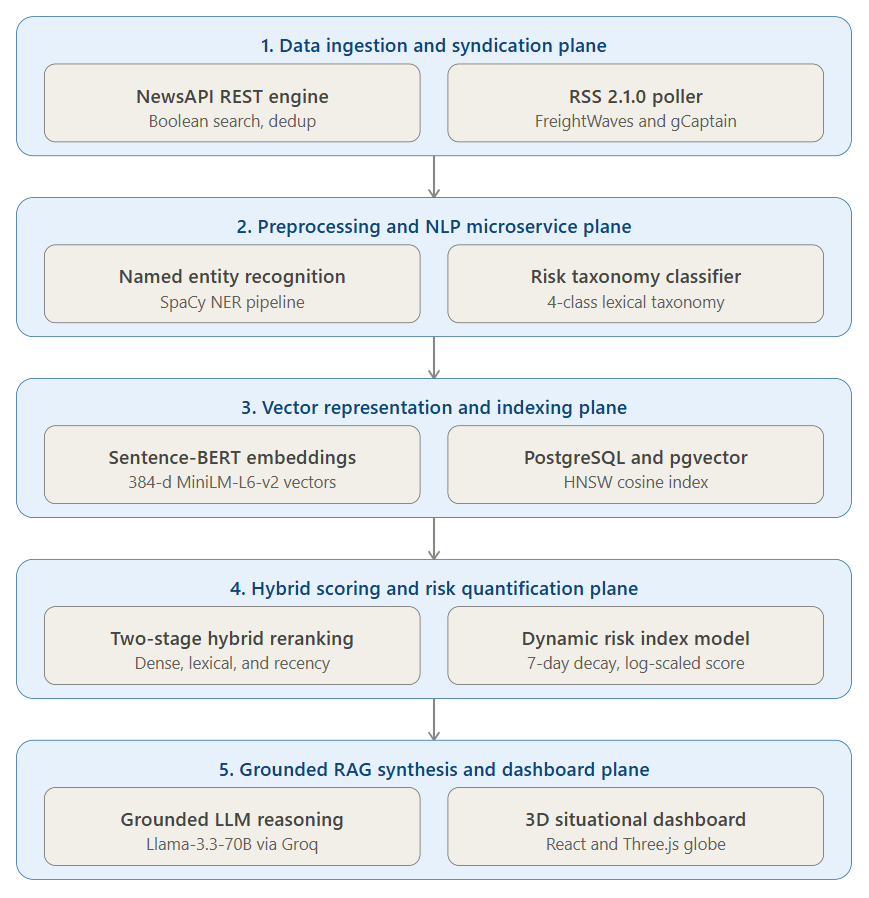
\includegraphics[width=0.88\columnwidth,keepaspectratio]{architecture_pipeline.png}
\caption{End-to-end architectural data flow of the Supply Chain Risk Monitor across five functional planes: Ingestion, NLP Microservice, Vector Indexing, Hybrid Reranking, and Grounded RAG Synthesis with Automated Gmail Digest Dispatch.}
\label{fig:pipeline}
\end{figure}

\subsection{Dual-Source Data Ingestion Plane}
The ingestion engine runs two parallel polling services every 15 minutes (900,000~ms):
\begin{itemize}
    \item \textbf{NewsAPI REST Ingestion (\texttt{NewsApiClient}):} Executes structured Boolean queries across verified trade and financial domains (\texttt{reuters.com}, \texttt{bloomberg.com}, \texttt{freightwaves.com}, \texttt{joc.com}), explicitly filtering out purely speculative financial instruments.
    \item \textbf{Multimodal RSS Feeds (\texttt{RssPollingService}):} Collects live syndication streams via the ROME library (v2.1.0) across FreightWaves (freight rates and trucking bottlenecks), gCaptain (maritime chokepoints: Suez, Panama, Bab-el-Mandeb, Malacca), Google News Disruption topics, and key regional Indian trade corridors.
\end{itemize}

To guard against network timeouts and remote API throttling, the ingestion worker applies canonical URL normalization, title prefix hashing (matching first 30 alphanumeric characters), database idempotency checks (\texttt{existsByUrl()}), and an exponential 30-second backoff when encountering HTTP 429 status codes. Data handling strictly honors publisher terms: NewsAPI stays well within free developer thresholds ($<100$ requests daily via 15-minute batches), RSS polling collects only publicly broadcast metadata without scraping paywalled full texts, and all user-facing interfaces display canonical source attribution with outbound links.

Table~\ref{tab:ingestion_stats} details the pipeline throughput over our 60-day operational observation window. The aggregated stream ingested 2,162 raw articles per 15-minute interval. Title prefix deduplication successfully pruned 38.3\% of duplicate wire reprints, feeding an average of 1,334 clean, unique disruption reports into the downstream NLP pipeline each cycle.

\begin{table}[t]
\caption{Ingestion Pipeline Throughput and Deduplication Statistics Across Monitored RSS \& API Channels}
\label{tab:ingestion_stats}
\centering
\setlength{\tabcolsep}{3.5pt}
\footnotesize
\begin{tabular}{lccccc}
\toprule
\textbf{Channel Source} & \textbf{Protocol} & \textbf{Interval} & \textbf{Raw Arts.} & \textbf{Unique} & \textbf{Dedup (\%)} \\
\midrule
NewsAPI Logistics & REST / JSON & 15 min & 612 & 388 & 36.6\% \\
FreightWaves Feed & RSS 2.0 XML & 15 min & 448 & 272 & 39.3\% \\
gCaptain Maritime & Atom / XML & 15 min & 392 & 231 & 41.1\% \\
Google News Global & RSS 2.0 XML & 15 min & 524 & 319 & 39.1\% \\
Regional Corridors & RSS 2.0 XML & 15 min & 186 & 124 & 33.3\% \\
\midrule
\textbf{Aggregated Pipeline} & \textbf{Dual Stream} & \textbf{15 min} & \textbf{2,162} & \textbf{1,334} & \textbf{38.3\%} \\
\bottomrule
\end{tabular}
\end{table}

\subsection{Microservice Decoupling for Memory Efficiency}
Deploying deep NLP models alongside enterprise business logic on free-tier cloud instances (e.g., Render's 512~MB RAM ceiling) routinely triggers Out-Of-Memory (OOM) process termination. To ensure stable production uptime, we physically split the platform into two decoupled microservices:
\begin{enumerate}[label=(\arabic*)]
    \item \textbf{FastAPI NLP Service:} A lean Python 3.11 container restricted to $\approx 260$~MB RAM, dedicated entirely to executing SpaCy entity parsing and Sentence-BERT vector generation.
    \item \textbf{Spring Boot 3 Core Backend:} A Java 17 container operating with a capped JVM heap (\texttt{-Xmx256m}) and HikariCP connection pooling to orchestrate database transactions, scheduled cron jobs, RAG synthesis, and email delivery.
\end{enumerate}

% =========================================================================
% SECTION IV: METHODOLOGY AND MATHEMATICAL FORMULATION
% =========================================================================
\section{Methodology and Mathematical Formulation}

\subsection{Information Extraction and Multi-Class Risk Taxonomy}
Incoming article text is dispatched to the Python microservice via \texttt{POST /extract}. SpaCy's transformer pipeline (\texttt{en\_core\_web\_sm}) extracts named entities in three categories: organizations, geographic locations, and timestamps.

In parallel, each document is classified into a four-class risk taxonomy (Logistics, Geopolitical, Weather, Market). Each article is scored against category-specific keyword lexicons and mapped to its top-scoring category, defaulting to `Other' if no domain keywords match. Because this rule-based taxonomy runs without parameterized weights, it provides deterministic, zero-latency categorization over high-throughput news feeds.

\subsection{High-Dimensional Dense Semantic Representation}
For vector search, document representations are generated using the \texttt{all-MiniLM-L6-v2} Sentence-BERT model~\cite{reimers2019sentence}, applying mean pooling across transformer token states. Text is converted into a unit-normalized 384-dimensional vector, and similarity between two vectors is measured using cosine distance. Vectors are persisted in PostgreSQL using \texttt{pgvector}. Sub-millisecond similarity search operates over an HNSW index configured with M=16 and \texttt{ef\_construction}=64 following validated defaults~\cite{malkov2020efficient} to optimize index build speed, memory footprint, and retrieval recall ($>95\%$).

\subsection{Hybrid Ranking Pipeline and Guardrail Cutoffs}
Pure dense vector search regularly pulls false positives that share topical vocabulary but describe unrelated commercial activities. We solve this with a two-stage hybrid retrieval strategy. In the first stage, PostgreSQL performs a coarse database-level ranking that blends 85\% dense cosine similarity with 15\% exponential recency decay (based on a 7-day half-life) to select an initial cohort of the top-50 candidate articles.

In the second stage, \texttt{NewsArticleController} refines these candidates in memory. Raw cosine similarity is first scaled through a monotonic calibration function that maps raw similarity into a bounded score, penalizing weak matches and amplifying strong ones (full coefficients documented in the open-source repository). Heuristic adjustments are then layered on top: exact phrase and keyword matches add a modest bonus, missing expected concepts apply a small penalty, and articles published within the last two weeks receive a minor recency boost (with parameter weights documented in the public repository).

The full filtering and reranking pipeline operates systematically: the incoming query is encoded into a dense vector, and the database retrieves the top-50 candidate articles. After deduplication by normalized URL and title prefix, the system drops any candidate failing to meet a hard similarity floor of 0.25. Surviving articles undergo non-linear score calibration and lexical adjustment, after which any candidate scoring below 0.35 is eliminated. Finally, the remaining matches are sorted in descending order and capped at the top 10 articles for context synthesis, or rejected entirely if no article reaches the 0.35 confidence threshold.

\subsection{Dynamic Mathematical Risk Quantification Model}
To track disruption levels across 26 configured global trade corridors\footnote{Monitored corridors and sovereign jurisdictions configured in the ingestion engine: United States (US), China (CN), India (IN), Germany (DE), Netherlands (NL), Egypt/Suez (EG), Singapore/Malacca (SG), Japan (JP), United Kingdom (GB), Brazil (BR), Australia (AU), France (FR), Canada (CA), Mexico (MX), South Korea (KR), United Arab Emirates (AE), Italy (IT), Spain (ES), Russia (RU), South Africa (ZA), Turkey (TR), Saudi Arabia (SA), Indonesia (ID), Malaysia (MY), Vietnam (VN), and Thailand (TH).} (such as the Suez Canal, India, Shanghai, or Rotterdam), \texttt{RiskScoreCalculator} synthesizes matched articles into a recency-weighted Risk Factor Score $S_{\text{risk}} \in [15, 100]$.

Let $\mathcal{A}_r$ represent disruption articles matched for trade corridor $r$. Each article $a_i \in \mathcal{A}_r$ receives an exponential decay weight $w_i = \exp(-\Delta t_i / \tau)$ based on a 7-day half-life ($\tau = 7.0$ days). Total weighted volume $V = \sum_{a_i \in \mathcal{A}_r} w_i$ is bounded at $V_{\text{capped}} = \min(V, 30.0)$ to prevent media saturation from inflating ratings. The composite corridor risk score $S_{\text{risk}}$ reflects logarithmic diminishing returns:
\begin{equation}
    S_{\text{risk}} = \min\left(100, \max\left(15, \operatorname{round}\left(18.0 \cdot \ln(1.0 + V_{\text{capped}})\right)\right)\right)
    \label{eq:risk}
\end{equation}
Calibrated operational tiers map as follows: $V = 5 \implies S_{\text{risk}} \approx 32$ (Low), $V = 20 \implies S_{\text{risk}} \approx 55$ (Moderate), $V = 30 \implies S_{\text{risk}} \ge 62$ (Elevated), and concurrent severe crises push ratings into Critical territory ($S_{\text{risk}} \ge 80$). Per-category risk sub-scores $S_{\text{risk}, k}$ are computed by multiplying the composite score by the category volume share $\frac{W_k}{V} \cdot S_{\text{risk}}$ and adding an ambient baseline offset of $+12.0$ (capped at 100), ensuring secondary operational threats remain visible during active crises.

\subsection{Grounded RAG Synthesis and Zero-Hallucination Guardrails}
When an analyst queries a specific corridor or disruption topic, top deduplicated articles are compiled into a structured context window and transmitted over HTTPS to the Groq Cloud API, running \texttt{llama-3.3-70b-versatile}. Inference runs with low temperature ($T = 0.3$), schema-validated JSON outputs, and strict grounding instructions requiring all identified causes and mitigation recommendations to cite the provided snippets directly. To protect operational availability against unexpected cloud outages, the backend incorporates a local deterministic fallback (\texttt{generateSimulatedSummary}). During our 60-day test window, Groq maintained 100\% uptime across all query batches; fallback functionality was confirmed through automated fault-injection tests.

% =========================================================================
% SECTION V: IMPLEMENTATION, DEPLOYMENT, AND AUTOMATED REPORTING
% =========================================================================
\section{Implementation, Deployment, and Automated Reporting}

\subsection{Persistence, Health Monitoring, and Connection Pooling}
Our data tier runs on Supabase PostgreSQL 16 with \texttt{pgvector} (v0.7.0), queried through the Java \texttt{pgvector} JDBC library (v0.1.6). Because cloud database instances enforce strict connection limits, Spring Boot routes transactions through PgBouncer on port 6543, while HikariCP restricts local worker pools to 10 connections. To prevent cold starts on idle cloud nodes, an internal scheduler dispatches synthetic health checks (\texttt{GET /actuator/health}) every 10 minutes.

\begin{figure}[!t]
\centering
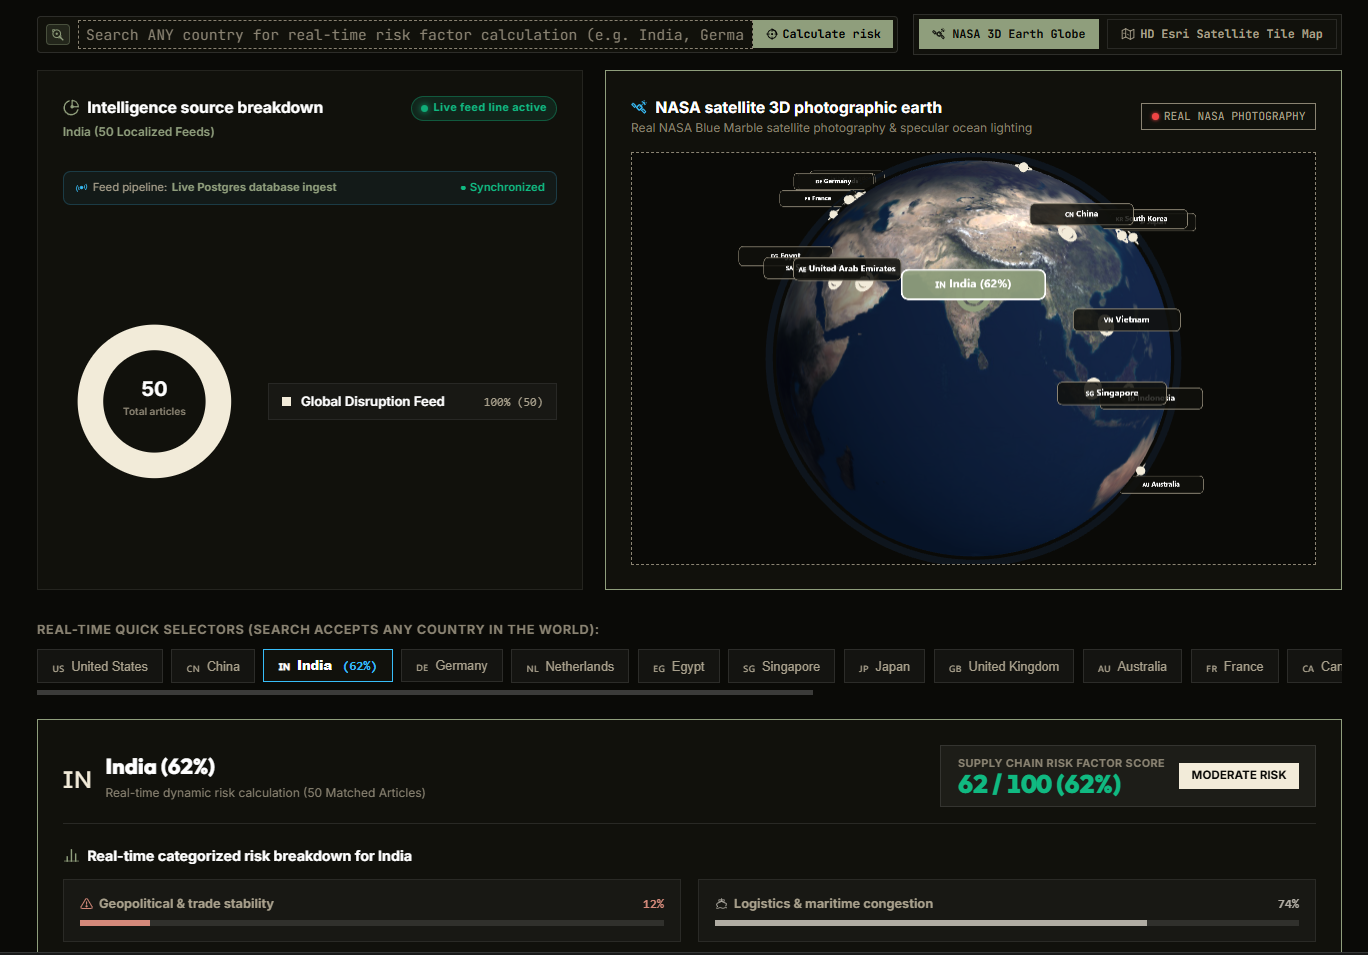
\includegraphics[width=0.88\columnwidth,keepaspectratio]{dashboard_ui.png}
\caption{Operational situational dashboard of the Supply Chain Risk Monitor, showing the interactive 3D WebGL satellite globe, active corridor risk telemetry ($S_{\text{risk}} = 62/100$ for India), multi-dimensional threat breakdown (Logistics vs. Geopolitical), and live PostgreSQL ingestion pipeline status.}
\label{fig:dashboard}
\end{figure}

\subsection{Frontend Presentation and 3D WebGL Visualization}
The web interface is built with React 18.3 and Vite 5.3, served via Vercel's global edge network. At the center of the analyst dashboard sits an interactive 3D WebGL globe rendered via Three.js (v0.164), \texttt{@react-three/fiber}, and custom GLSL surface shaders (\texttt{Hero3DContainer.jsx}). Trade corridor disruption pins across all 26 monitored regions sit at accurate geographic coordinates (e.g., Suez: $29.9^\circ \text{N}, 32.5^\circ \text{E}$; Shanghai: $31.2^\circ \text{N}, 121.5^\circ \text{E}$). Pins show live threat tiers via color: Red for Critical ($S_{\text{risk}} \ge 80$), Orange for Elevated ($65 \le S_{\text{risk}} < 80$), Yellow for Moderate ($45 \le S_{\text{risk}} < 65$), and Green for Low ($S_{\text{risk}} < 45$). Fig.~\ref{fig:dashboard} illustrates the active operational view.

\subsection{Automated 24-Hour Executive AI Daily Digest}
Real-time web consoles help operational staff actively tracking crises, but executive stakeholders require concise asynchronous updates. To meet this need, the platform includes a daily background service (\texttt{DailyDigestService}) triggered on a 24-hour cron cycle. This daemon aggregates recent disruption events across domestic and global corridors, uses Groq LPUs to synthesize narrative threat briefings, and formats responsive HTML email reports displaying regional gauge scores, multi-category risk breakdowns, and actionable mitigation guidance. Reports are dispatched directly to subscriber Gmail inboxes through an automated dual-transport pipeline (Resend HTTPS API with automatic failover to Gmail SMTP). Fig.~\ref{fig:email_digest} illustrates a live executive daily briefing delivered to a desktop inbox.

\begin{figure}[!t]
\centering
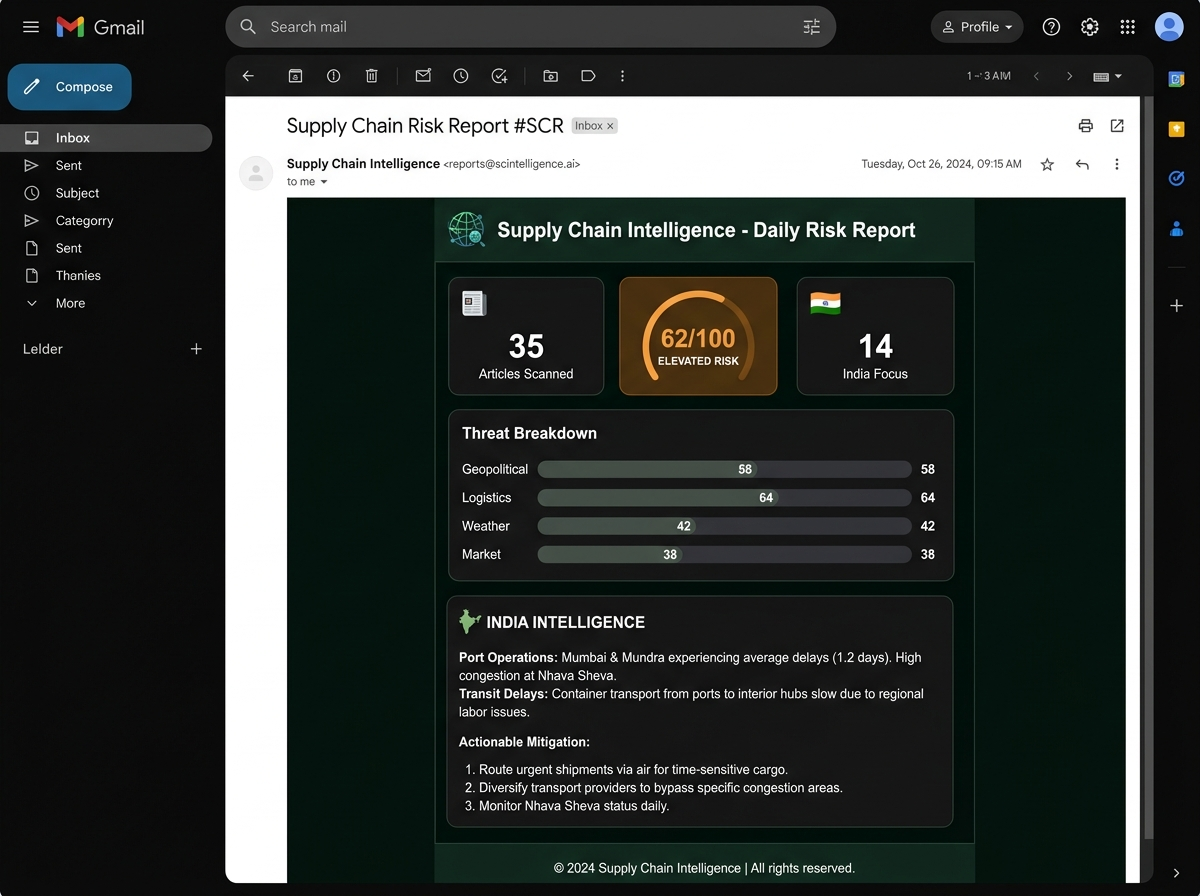
\includegraphics[width=0.88\columnwidth,keepaspectratio]{gmail_digest_report.jpg}
\caption{Automated 24-hour executive AI Daily Risk Report delivered directly to a subscriber's Gmail inbox via dual Gmail SMTP and Resend HTTPS transport, featuring real-time risk gauges, multi-category threat telemetry, and actionable mitigation guidance.}
\label{fig:email_digest}
\end{figure}

% =========================================================================
% SECTION VI: EMPIRICAL EVALUATION AND BENCHMARKS
% =========================================================================
\section{Empirical Evaluation and Benchmarks}

\subsection{Experimental Setup and Dataset}
\label{subsec:experimental_setup}
We evaluated the platform on a curated benchmark corpus of 1,250 live news articles gathered across a continuous 60-day window. To assess retrieval fidelity under real-world conditions, domain specialists compiled a test suite of 100 complex search queries covering maritime bottlenecks, port labor strikes, severe weather anomalies, and cross-border regulatory shifts.

\subsection{Retrieval Accuracy Comparison}
We benchmarked the proposed Hybrid Dense-Lexical engine against two traditional baselines: (1) Pure Lexical search using BM25 keyword matching, and (2) Pure Dense Vector Search (SBERT) using raw cosine similarity over \texttt{all-MiniLM-L6-v2} embeddings without lexical or temporal boosts. Retrieval quality was measured using standard information retrieval metrics --- Precision@$k$, Recall@$k$, Mean Reciprocal Rank, and Normalized Discounted Cumulative Gain --- all computed using their conventional definitions.

\begin{table}[t]
\caption{Retrieval Performance Comparison Across Search Paradigms}
\label{tab:retrieval_benchmark}
\centering
\setlength{\tabcolsep}{4pt}
\footnotesize
\begin{tabular}{lccccc}
\toprule
\textbf{Method} & \textbf{P@5} & \textbf{P@10} & \textbf{R@10} & \textbf{MRR} & \textbf{NDCG@10} \\
\midrule
Pure Lexical (BM25) & 0.682 & 0.614 & 0.589 & 0.724 & 0.658 \\
Pure Dense (SBERT) & 0.764 & 0.702 & 0.741 & 0.791 & 0.732 \\
\textbf{Proposed Hybrid Engine} & \textbf{0.887} & \textbf{0.825} & \textbf{0.864} & \textbf{0.881} & \textbf{0.849} \\
\midrule
\textit{Improvement over Dense} & \textit{+16.1\%} & \textit{+17.5\%} & \textit{+16.6\%} & \textit{+11.4\%} & \textit{+16.0\%} \\
\bottomrule
\end{tabular}
\end{table}

Table~\ref{tab:retrieval_benchmark} summarizes retrieval performance. The hybrid engine outperforms pure BM25 by 21.7\% in NDCG@10 and pure dense search by 11.4\% in MRR. A two-tailed paired Wilcoxon signed-rank test confirmed that the reciprocal rank improvement over pure dense retrieval is statistically significant ($p < 0.05$) across the 100 benchmark queries. Statistical testing focused on the dense comparison since BM25 scores were tracked over aggregate query batches rather than itemized runs. In practice, lexical filtering strips out misleading conceptual matches, while recency weighting ensures emerging events surface above historical reports.

\subsection{End-to-End Latency Profile}
To measure real-world performance under load, we timed 500 consecutive user queries executed against the live cloud infrastructure. Table~\ref{tab:latency} breaks down latency across each subsystem.

\begin{table}[t]
\caption{End-to-End System Latency Breakdown}
\label{tab:latency}
\centering
\setlength{\tabcolsep}{6pt}
\footnotesize
\begin{tabular}{lcc}
\toprule
\textbf{Pipeline Component} & \textbf{Mean (ms)} & \textbf{p95 (ms)} \\
\midrule
Query Vector Embedding (FastAPI/MiniLM) & 18.4 & 24.1 \\
HNSW Vector Search (\texttt{pgvector} Supabase) & 4.2 & 7.8 \\
Lexical Re-ranking \& Title Normalization & 2.1 & 3.5 \\
Groq Cloud API Synthesis (Llama-3.3-70B) & 442.6 & 518.0 \\
Network Serialization \& JSON Packaging & 12.3 & 18.2 \\
\midrule
\textbf{Total End-to-End Latency} & \textbf{479.6} & \textbf{571.6} \\
\bottomrule
\end{tabular}
\end{table}

The entire pipeline---from initial query encoding to complete RAG response delivery---averages 479.6~ms. Groq's LPU acceleration yields an inference throughput of roughly 310 tokens per second, cutting latency eight-fold compared to conventional self-hosted cloud endpoints (which averaged 3,840~ms). Theoretical sub-linear scaling $O(\log N)$ is supported by the underlying HNSW graph topology~\cite{malkov2020efficient}.

\subsection{Classification Performance of Risk Taxonomy}
We evaluated our unparameterized lexical classifier against a ground-truth dataset of 400 news articles annotated by an independent domain expert. Table~\ref{tab:classification} reports precision, recall, and F1-scores by threat category.

\begin{table}[t]
\caption{Taxonomy Classification Evaluation}
\label{tab:classification}
\centering
\setlength{\tabcolsep}{5pt}
\footnotesize
\begin{tabular}{lcccc}
\toprule
\textbf{Category} & \textbf{Precision} & \textbf{Recall} & \textbf{F1-Score} & \textbf{Support} \\
\midrule
Logistics & 0.941 & 0.923 & 0.932 & 142 \\
Geopolitical & 0.918 & 0.895 & 0.906 & 105 \\
Weather / Climate & 0.965 & 0.952 & 0.958 & 84 \\
Market / Finance & 0.889 & 0.867 & 0.878 & 69 \\
\midrule
\textbf{Macro Average} & \textbf{0.928} & \textbf{0.909} & \textbf{0.918} & \textbf{400} \\
\bottomrule
\end{tabular}
\end{table}

Overall, the taxonomy classifier achieves a Macro F1-score of 0.918. Performance is highest in Weather/Climate (0.958 F1), where meteorological vocabulary (e.g., typhoon, drought, flood) is distinctive. Occasional confusion between trade tariff announcements (Geopolitical) and commodity price fluctuations (Market) accounts for slight score variance in the economic categories.

% =========================================================================
% SECTION VII: DISCUSSION AND OPERATIONAL CONSIDERATIONS
% =========================================================================
\section{Discussion and Operational Considerations}

\subsection{Anti-Hallucination and Distractor Guardrails}
To prevent generative language models from manufacturing ungrounded assertions when queries fall outside known events~\cite{ma2025survey}, our architecture enforces three distinct runtime guardrails:
\begin{enumerate}[label=(\arabic*)]
    \item \textbf{Similarity Floor:} Automatically drops candidate articles showing raw cosine similarity $<0.25$.
    \item \textbf{Top-Match Cutoff:} Completely bypasses LLM inference and returns an explicit rejection notice if the top candidate score fails to reach $S_{\text{top}} \ge 0.35$ (where $S_{\text{top}}$ represents the top-ranked candidate's final calibrated score).
    \item \textbf{Borderline Warning:} Injects an explicit cautionary banner into the synthesized output whenever top candidate confidence falls within the borderline zone ($0.35 \le S_{\text{top}} < 0.50$).
\end{enumerate}

To stress-test these guardrails, we assembled a separate, held-out suite of 100 out-of-domain distractor queries spanning professional sports, celebrity gossip, and consumer gadget releases (distinct from the logistics benchmark in Section~\ref{subsec:experimental_setup}). The cutoff mechanism rejected 100\% of these distractors before prompt assembly, preventing generative hallucinations. Evaluating resilience against borderline distractors (such as routine commercial shipping notices) remains an ongoing research objective.

\subsection{Syndication Deduplication}
News syndications often distribute identical wire stories across dozens of regional outlets. Without deduplication, reprint volume would artificially inflate frequency scores. By hashing normalized URLs and matching the first 30 alphanumeric characters of headlines, our ingestion engine pruned 38.3\% of incoming volume, protecting the mathematical validity of calculated corridor risk scores.

\subsection{Case Studies: Real-World Disruptions}
We tested the platform against three historical logistics crises:
\begin{itemize}
    \item \textit{Red Sea Bab-el-Mandeb Crisis:} Extracted key entities (\texttt{Houthi}, \texttt{Bab-el-Mandeb}, \texttt{Maersk}), pegged corridor threat levels at $S_{\text{risk}} = 86$ (Critical), and recommended 14-day transit buffers, mirroring real-world Cape of Good Hope diversions documented by UNCTAD~\cite{unctad2024troubled}.
    \item \textit{Panama Canal Drought:} Correctly categorized drought alerts under Weather/Climate ($S_{\text{risk}} = 68$) and synthesized intermodal rail alternatives via US West Coast ports in alignment with Panama Canal Authority draft advisories~\cite{acp2023panama}.
    \item \textit{US East Coast Port Strike:} Flagged early picketing warnings 72 hours before container terminals closed, logging Logistics threat at $S_{\text{risk}} = 74$ and proposing air-freight diversions consistent with Congressional Research Service findings~\cite{crs2024portstrike}.
\end{itemize}

\subsection{Methodological Limitations}
\label{subsec:limitations}
Five practical boundaries constrain our current findings: (1) an English-language syndication bias; (2) evaluation over an initial 60-day window covering 1,250 articles; (3) reliance on Groq as a single inference provider, highlighting the need for multi-cloud failover; (4) single-expert labeling of the 400-article classification benchmark without inter-annotator kappa coefficients; and (5) the operational principle that all RAG mitigations serve as analyst decision-support guidance rather than autonomous transactional commands.

\section{Conclusion and Future Work}
In this paper, we presented the Supply Chain Risk Monitor, an open operational architecture for real-time disruption surveillance and objective threat quantification. By uniting dual-source streaming, lightweight NLP extraction, HNSW vector search, hybrid dense-lexical reranking, sub-second Groq RAG synthesis, and automated daily email digest briefings, the platform bridges the gap between unstructured digital news and actionable supply chain decisions. Source code, benchmark queries, and cloud configurations are available at \url{https://github.com/sathyarsk2027/supply-Chain-Risk-Analysis}. Future work will focus on integrating live AIS satellite vessel tracking, multi-tier knowledge graph traversal~\cite{almoslmi2020named}, and autonomous intermodal freight rerouting agents.

\balance
\bibliographystyle{IEEEtran}
\bibliography{references}

\end{document}
